%Autores: Cassiopea Acebes Prado
%Contato: cassiopea.acebes@gmail.com
%"Modelo para escrita de artigos científicos para o TCC dos cursos Graduação do INATEL - Instituto Nacional de Telecomunicações."

%paquetes que se van a usar, a parte del documentclass
\documentclass[12pt,twocolumn]{article}
\usepackage{graphicx}
\usepackage[spanish]{babel}
\usepackage[utf8x]{inputenc}
\usepackage{fancyhdr}
\usepackage{listings}
\usepackage{float}
\usepackage{mathtools}
\renewcommand{\footrulewidth}{0.1pt} %Esto hace la barra de abajo
\setlength\headheight{16pt} %Para evitar el error \headheight is too small

\graphicspath{{img/}} %Toma imágenes de la carpeta img

\usepackage[dvipsnames]{xcolor}
\definecolor{backcolour}{rgb}{0.95,0.95,0.92}
\lstdefinestyle{mystyle}{
    backgroundcolor=\color{backcolour},
    basicstyle=\ttfamily\footnotesize,
    breakatwhitespace=false,
    breaklines=true,
    keepspaces=true,
    showspaces=false,
    showstringspaces=false,
    showtabs=false,
    tabsize=2
}
\usepackage[T1]{fontenc}
\lstset{style=mystyle, escapeinside=||}

\pagestyle{fancy}
\fancyhf{}
\fancyhead[L,RO]{28/02/2022}
\fancyhead[R]{pelocarioca\_}

\fancyfoot[L,LO]{Cassiopea Acebes Prado}
\fancyfoot[R,RO]{Página \thepage}


\begin{document}
\onecolumn
\title{\Huge \bf Apartado técnico y especificaciones para Manual para el topoanálisis del hogar}

\author{Cassiopea Acebes Prado}

\maketitle


%índice
\tableofcontents

\newpage
\twocolumn
\section{Introducción}

En este documento se recoge la documentación técnica de la obra \textit{Manual para el topoanálisis del hogar} para la pieza \textit{Manual para el topoanálisis del hogar}, independientemente de su formato, para la generación, disposición, proyección y control de la proyección de las normas.

También incluye una serie de recomendaciones (Sección \textit{Recomendaciones}) y anexos fotográficos y de código (Sección \textit{Resultados}). Estos se utilizarán para explicar el funcionamiento normal de los componentes; para dar posibles adaptaciones de cara a la instalación física de la pieza; facilitar la cita, referencia o mención de la documentación técnica, diseño o funcionamiento de los componentes; y posibilitar la recuperación de piezas de código para su uso en la instalación.

	
\section{Desarrollo}
	\subsection{Proceso Generación normas}
	
	\subsubsection{Introducción}
	En esta subsección se va a documentar el software para la generación de las normas de la pieza \textit{Manual para el topoanálisis del hogar}. Se tratarán los requisitos del componente, su funcionamiento y sus dos salidas, en la Sección de \textit{Resultados} se adjuntará una copia del código básico.
	
	\subsubsection{Requisitos}
	Este componente debe hacer lo siguiente:
	\begin{itemize}
	\setlength\itemsep{-0.3em}
	\item Tomar como \textit{input} las normas recopiladas.
	\item Generar, a partir de las normas originales, nuevas normas.
	\item Dar una salida por escrito y por vídeo de las nuevas.
	\end{itemize}
	
	Se debe tener en cuenta que las nuevas normas	 son de naturaleza aleatoria, es decir que no tienen que tener un sentido lógico, y que se pueden adaptar las normas originales para poderse utilizar en el \textit{software}.
	
	\subsubsection{Funcionamiento}

	Las normas recopiladas pasan por un proceso de normalización para su posterior procesamiento, para ello se determina una fórmula general o estructura sintáctica. Esta fórmula se utiliza en todos los puntos del procesamiento, se compone de:\\
	
	\textbf{Adv.Neg. + verbo + sujeto + CCL + CCT + CCM + Consecuencia}\\
	
	Donde \textbf{Adv.Neg.} se trata de un adverbio de negación, \textbf{CCL} de un complemento circunstancial de lugar, \textbf{CCT} un complemento circunstancial de tiempo, \textbf{CCM} un cc de modo y \textbf{consecuencia} una estructura que actúa como consecuencia a la norma. No todas las normas contienen todos los componentes, por lo que se permite que haya componentes vacíos.\\
	
	Una vez tomadas las partes de las normas recopiladas, estas pasan por una doble selección aleatoria. En primer lugar se selecciona una estructura sintáctica para la nueva norma, a las diferentes estructuras se las llama \textit{seeds} y contienen variaciones de la estructura original, añadiendo o quitando componentes.
	Una vez hecha la selección de la estructura de los componentes, cada uno de ellos se selecciona aleatoriamente. Esto permite que se genere una variedad ciertamente orgánica a las normas generadas, algunos ejemplos de las \textit{seeds} son:
	\begin{lstlisting}[texcl=true]
negacion + verbo + sujeto + ccl 
negacion + verbo + consecuencia
negacion + verbo + sujeto + ccl + ccm
	\end{lstlisting}
	
	Se explica línea por línea el código del componente, realizado en \textit{Python} en su versión 3.8.5:

	

Para poder elegir números aleatorios, y de esta forma seleccionar las partes de
las normas aleatoriamente, se requiere de un módulo específico llamado 'secrets'.
Se le llama con la línea 8 y para utilizar sus funciones se le trata como
un objeto.
\begin{lstlisting}[texcl=true]
import secrets
\end{lstlisting}

Se van a generar archivos con normas, para que cada vez que se ejecute el generador
no se sobreescriba el anterior archivo se incluirá la fecha y hora en que se crearon.
Para esto se utiliza el módulo 'datetime', que puede dar la fecha y hora momentáneamente.
\begin{lstlisting}[texcl=true]
import datetime
\end{lstlisting}

Se toman las variables para construir las frases, para ello se lee un archivo y
se forma un array (una 'lista') con las líneas de texto de cada archivo.

Las líneas de lectura de los archivos tienen tres partes:
	\begin{itemize}
	\setlength\itemsep{-0.3em}
    \item \textbf{negacion =} \\
    Se asigna el array de la lectura del archivo a la variable 'negacion'.
    \item \textbf{open('partes-normas/negacion','r')} \\
    Lee el archivo 'negacion' de la carpeta 'partes-normas'.
    \item \textbf{.read().splitlines()} \\
    Asigna cada línea del archivo a un ítem del array.
	\end{itemize}
De esta forma la variable 'negacion' terminaría funcionando como:\\


negacion['no', 'jamás',(...)]\\


	
Aligerando así el código del generador

\begin{lstlisting}[language=python]
negacion = open('partes-normas/negacion','r').read().splitlines()
verbo = open('partes-normas/verbo','r').read().splitlines()
sujeto = open('partes-normas/sujeto','r').read().splitlines()
ccl = open('partes-normas/ccl','r').read().splitlines()
cct = open('partes-normas/cct','r').read().splitlines()
ccm = open('partes-normas/ccm','r').read().splitlines()
consecuencia = open('partes-normas/consecuencia','r').read().splitlines()
\end{lstlisting}

Para hacer más visual el código, se va a crear un alias de la función 'choice()'
del módulo secrets llamado 'random()', así cada vez que se quiera seleccionar un
elemento aleatorio de un array de datos aparecerá como 'random(y)' en vez de como
'secrets.choice(y)'. Esto es puramente visual.
\begin{lstlisting}[texcl=true]
def random(a):
    return secrets.choice(a)
\end{lstlisting}

Ahora se definen las funciones que actúan como seeds, cada seed es una estructura
de normas, de esta forma las seeds (denominadas seed0, seed1,...seed10) tienen
diferentes componentes, como una negación, un complemento circunstancial de un tipo
u otro o una consecuencia. De esta forma se crean frases con diversas estructuras,
lo que hace menos repetitivas las normas.

El funcionamiento de una seed N es el siguiente:
	\begin{itemize}
	\setlength\itemsep{-0.3em}
    \item \textbf{def seedN(): }\\ Es la declaración de la función.
    \item  \textbf{x='' } \\ Inicializa la variable x, en la que se añadirán las partes de la norma.
    \item \textbf{x += random(negacion) + ' ' } \\ Añade a la variable x vacía una negación aleatoria y añade un espacio.
    \item \textbf{x += random(verbo) + ' ' } \\ Añade a la negación y al espacio un verbo aleatorio con un espacio delante.
    \item \textbf{x += random(sujeto) + ' ' } \\ Añade a la negación y al verbo un sujeto. Añade un espacio delante, aunque no es necesario.
    \item \textbf{return x.strip('\_ ') } \\ Devuelve la norma guardada en la variable x, le quita un posible '\_' del archivo de negaciones. Al devolver la variable esta se convierte en la salida de la funcion, es como si fuera su resultado.
	\end{itemize}
Se pueden añadir y quitar partes a las seeds para dar variedad a las frases.
\begin{lstlisting}[texcl=true]
def seed0():
    x=''
    x += random(negacion) + ' '
    x += random(verbo) + ' '
    x += random(sujeto) + ' '
    x += random(ccl) + ' '
    x += random(cct) + ' '
    x += random(ccm) + ' '
    x += random(consecuencia) + ' '
    return x.strip('\_ ')


def seed1():
    x=''
    x += random(negacion) + ' '
    x += random(verbo) + ' '
    x += random(sujeto) + ' '
    return x.strip('\_ ')


def seed2():
    x=''
    x += random(negacion) + ' '
    x += random(verbo) + ' '
    x += random(sujeto) + ' '
    x += random(ccl) + ' '
    x += random(ccm) + ' '
    return x.strip('\_ ')

def seed3():
    x=''
    x += random(negacion) + ' '
    x += random(verbo) + ' '
    x += random(sujeto) + ' '
    return x.strip('\_ ')

def seed4():
    x=''
    x += random(negacion) + ' '
    x += random(verbo) + ' '
    x += random(sujeto) + ' '
    x += random(cct) + ' '
    x += random(ccm) + ' '
    return x.strip('\_ ')

def seed5():
    x=''
    x += random(negacion) + ' '
    x += random(verbo) + ' '
    x += random(consecuencia) + ' '
    return x.strip('\_ ')

def seed6():
    x=''
    x += random(negacion) + ' '
    x += random(verbo) + ' '
    x += random(sujeto) + ' '
    x += random(cct) + ' '
    return x.strip('\_ ')

def seed7():
    x=''
    x += random(negacion) + ' '
    x += random(verbo) + ' '
    x += random(sujeto) + ' '
    x += random(ccm) + ' '
    return x.strip('\_ ')

def seed8():
    x=''
    x += random(negacion) + ' '
    x += random(verbo) + ' '
    x += random(sujeto) + ' '
    x += random(ccm) + ' '
    return x.strip('\_ ')

def seed9():
    x=''
    x += random(negacion) + ' '
    x += random(verbo) + ' '
    x += random(sujeto) + ' '
    x += random(ccl) + ' '
    x += random(cct) + ' '
    return x.strip('\_ ')

def seed10():
    x=''
    x += random(negacion) + ' '
    x += random(sujeto) + ' '
    x += random(ccl) + ' '
    x += random(cct) + ' '
    x += random(ccm) + ' '
    return x.strip('\_ ')
\end{lstlisting}

Ahora se crea el nombre del archivo, que tendrá la estructura:\\

output-YYYY-MM-DD\_HH.MM.SS.mmmmm.txt\\


\begin{itemize}
\setlength\itemsep{-0.3em}
\item \textbf{'generadas/output-'}\\
 Guarda en la carpeta 'generadas', el nombre del archivo comienza por 'output'.
\item \textbf{str(datetime.datetime.now()).replace(' ', '\_').replace(':', '.')}\\
 Obtiene la fecha y hora y las formatea.
\item \textbf{'.txt'}\\
 Terminación del archivo, al ser este de texto.
\end{itemize}
En la siguiente línea a la de la inicialización de nombre\_archivo se 'crea'
(abre) un archivo vacío con ese nombre, la opción 'w' indica que se va a escribir.
\begin{lstlisting}[texcl=true]
nombre\_archivo = 'generadas/output-'+str(datetime.datetime.now()).replace(' ', '\_').replace(':', '.')+'.txt'
output = open(nombre\_archivo, 'w')
\end{lstlisting}
Ahora se utiliza un bucle para que se añadan 50 normas generadas aleatoriamente
al archivo abierto. Ahora se explicarán las partes de la línea de output.(...):
\begin{itemize}
\setlength\itemsep{-0.3em}
\item \textbf{output.write(...)}\\
Lo que se encuentre dentro del paréntesis se va a escribir en el archivo abierto.

\item \textbf{locals()[...]() + '\textbackslash n'}\\
    locals() se trata de una 'lista' con las funciones del programa, entre otras funciones de python se encuentran las seeds. Para seleccionar una seed en concreto se utilizan los corchetes, de forma que entre ellos se escribe el nombre de la función que se quiera utilizar. Si a este locals()[...] se le añade un paréntesis '()', se ejecutará la función que se haya escrito en los corchetes. Por ejemplo 'locals()[seed5]()' ejecutará la función seed5().  Esto se utiliza porque interesa que lo que se ejecute (lo que hay entre los corchetes) sea aleatorio. Y esto es más sencillo si se llama a la seed desde locals(). Por último, el (+ '\textbackslash n')  sirve para que haya un salto de línea al final de cada norma.

\item \textbf{'seed' + str(secrets.randbelow(11))}\\
     Esto es lo que se encontraría dentro de los corchetes, de igual forma que con el nombre del archivo se le añade a la palabra 'seed' un número aleatorio por debajo de 11. Este número debe ser convertido a formato texto para poderse adjuntar a seed, de ahí que se utilice el str(...).

\end{itemize}
En conclusión, por cada iteración del bucle se añade al archivo el 'resultado'
(la norma correspondiente) de una de las funciones seed. Siendo esta elegida
aleatoriamente.
\begin{lstlisting}[texcl=true]
for i in range(50):
    output.write(locals()['seed' + str(secrets.randbelow(11))]()+'\textbackslash n')
\end{lstlisting}

Por último, se cierra el archivo abierto con close(). Esto se suele utilizar
para que en archivos grandes la memoria del ordenador no se sobrecargue, en este
caso no resulta del todo necesario pero se trata de una buena práctica de programación.
\begin{lstlisting}[texcl=true]
output.close()
\end{lstlisting}


	
	\subsubsection{Salidas}
	
	Para este componente existen dos salidas; una en forma de archivo de texto, considerada como la predeterminada, que crea el archivo que referencia el código anterior con cincuenta (50) normas; y una salida por consola, utilizada en la proyección de las normas en conjunto con el siguiente componente (Subsección \textit{Proceso Proyección Manual}).
	
	Para este segundo componente se sustituirían las dos últimas líneas (que referencian a la creación de un archivo) por esto:
	\begin{lstlisting}[texcl=true]
	for i in range(20000):
    		locals()['seed' + str(secrets.randbelow(11))]()+"\n"
\end{lstlisting}

Esta pieza de código hace que se ejecute la función \textit{seedX}, con X un número aleatorio, y añada al final de cada ejecución un salto de línea. Se requiere también de añadir la siguiente línea a cada función de \textit{seed}, para que la nueva norma salga por consola.
\begin{lstlisting}[texcl=true]
print(x.strip("_ "))
\end{lstlisting}  	
\newpage
	\subsection{Proceso Proyección normas}
	
	\subsubsection{Introducción}
	En esta subsección se va a documentar el software y el montaje del hardware para la proyección de las normas de la pieza \textit{Manual para el topoanálisis del hogar}. Se tratarán los requisitos del componente, su montaje y el funcionamiento de su \textit{software} en la Sección de \textit{Resultados} se adjuntará una copia del código y pictogramas del montaje.
	
	\subsubsection{Requisitos}	
	Este componente debe poder hacer lo siguiente:
	\begin{itemize}
	\setlength\itemsep{-0.3em}
	\item Detectar personas en una determinada zona (zona de detección ó ZDD).
	\item En caso de detectar a alguien en la ZDD, abrir el paso a la luz de un proyector.
	\item Cuando deje de detectar a alguien, cerrar el paso de la luz del proyector.
	\end{itemize}
	
	Por las características del proyector este componente es puramente de hardware, haciendo uso de una PLC Arduino Uno con los módulos de Servo Motor SG90, Sensor ultrasonidos HC-SR04 y una placa de pruebas modular. 
	
	\subsubsection{Funcionamiento}

Para la proyección de las normas se va a utilizar un proyector estándar configurado para dar la salida del Generador de normas por consola. La imagen que va a tener el proyector es una fuente de vídeo con texto integrado, el cual se va generando dinámicamente. Para abrir y cerrar la imagen se va a utilizar un trozo rectangular (o de una forma similar para mejorar la absorción de luz) de cartulina negra. Este trozo de cartulina irá montada en el servo, que se accionará con la arduino y el sensor. 

Para unir los distintos métodos se utilizará la placa de pruebas (\textit{protoboard}), conectándose mediante cables macho-macho de la siguiente forma (una 'pista' es una de las filas de la placa):

	\begin{itemize}
	\setlength\itemsep{-0.5em}
	\item Pista 1:
		\begin{itemize}
		\setlength\itemsep{-0.3em}
		\item Arduino: +5V.
		\item Sensor: VCC.
		\item Servo: Cable Rojo.
		\end{itemize}
	\item Pista 2:
		\begin{itemize}
		\setlength\itemsep{-0.3em}
		\item Arduino: Gnd.
		\item Sensor: Gnd.
		\item Servo: Cable Marrón.
		\end{itemize}		
	\item Pista 3:
		\begin{itemize}
		\setlength\itemsep{-0.3em}
		\item Arduino: D3.
		\item Sensor: Trig.
		\end{itemize}	
	\item Pista 4:
		\begin{itemize}
		\setlength\itemsep{-0.3em}
		\item Arduino: D2.
		\item Sensor: Echo.
		\end{itemize}	
	\item Pista 5:
		\begin{itemize}
		\setlength\itemsep{-0.3em}
		\item Arduino: D7.
		\item Servo: Cable amarillo.
		\end{itemize}	
	\end{itemize}
	

También se debe de resolver el problema de la detección, este problema de apariencia sencilla tiene infinidad de soluciones, desde la más elemental; limitarse a detectar algo cuando pasa de cierta distancia (x < d), hasta el uso de múltiples sensores e incluso cámaras. La solución que se ha apostado es la de utilizar un cierto rango de sensibilidad, a efectos de evitar las detecciones por ruido, que permite hacer detecciones cuando la distancia detectada se sale de este rango. Dado:\\

d $\rightarrow$ distancia a la pared, o la distancia detectada base

x $\rightarrow$ distancia leída en cada iteración (se supone que esta función se ejecuta todo el rato en bucle)

p $\rightarrow$ permisividad de la fórmula, permite establecer un rango en el que la detección se mantenga nula (reduce el movimiento errático del brazo).

Se utiliza la siguiente fórmula para la detección de personas u objetos:

$s=\left(\frac{x-d}{p}\right)^{2}\begin{cases}
s<1 & False\\
s>=1 & True
\end{cases}$\\ Donde False es que no hay detección y True que detecta un cuerpo.

El cociente (s) es el que determina la detección. Si (s) es inferior a 1, se considera que no hay nada/nadie en la zona de detección; si (s) es igual o mayor que 1, se considera que hay un objeto o persona en la zona de detección. Esta aproximación a una detección efectiva utiliza el cuadrado del valor para añadirle sensibilidad al resultado sin reducir la velocidad del cálculo, que es lo que interesa en este detector.

Para la obtención de los casos del cociente (s) y el divisor interno se ha calculado que a una distancia base de 300cm, considerando una diferencia de ruido de +-10cm, no hay nadie siendo detectado. Esta fórmula funciona tanto si hay alguien que de alguna forma cancele el ruido (caso x -> ∞) como si este alguien se encuentra muy cerca del detector (caso x < 300+-10cm).\\

Se expone el código del programa que hace funcionar el detector y el servo:\\

Se definen los pines que se van a 
utilizar y se declaran las variables
globales, también se incluye la 
librería de control del servo:

\begin{lstlisting}[texcl=true]
#include <Servo.h>

#define echoPin 2 // Pin D2 (Echo)
#define trigPin 3 // Pin D3 (Trig)
#define servPin 7 // Pin D7 (Serv)

long duration; // Tiempo de viaje del sonido
int distancia; // Distancia detectada en cada instante

long s; // Cociente del detector
int base = 1184; // Distancia base del detector (zona de detecci|ón vací|a)
int permisividad = 20; //Varianza de la distancia
int giro = 90; // Grados de giro del servo
int giro = 50; // Grados de giro del servo

\end{lstlisting}

Esta línea inicia el servo en la vabiable
servo, que se utilizará para su control:

\begin{lstlisting}[texcl=true]
Servo servo;
\end{lstlisting}

Se comienzan las salidas por consola 
  por el el terminal serial, de esta forma
  se podrán ver y analizar las lecturas que 
  tome el sensor, el estado del servo y otra 
  información de relevancia:
  
\begin{lstlisting}[texcl=true]
void setup() {
  Serial.begin(9600);
\end{lstlisting}

Para la toma de medidas se declaran los
  Pins del sensor como de salida y entrada
  y se le asigna al servo el pin definido
  
  El brazo del servo se pone a cero:
  
\begin{lstlisting}[texcl=true]
  pinMode(trigPin, OUTPUT); // Sets the trigPin as an OUTPUT
  pinMode(echoPin, INPUT); // Sets the echoPin as an INPUT
  servo.attach(servPin); //Servo al pin declarado

  servo.write(0); //Hace el cero del brazo del servo
  
}
\end{lstlisting}

Se declara el loop principal
del programa, en este se va a 
primero tomar una medida por media, 
se le declara al valor 'average' el
resultado de la media, luego se toma
una medida real y se calcula el estado 
del brazo, en caso de ser positivo 
subir; en caso negativo, bajará.

Se hace una impresión por el monitor
del estado del sensor, esto ayudará
a la depuración y al ajuste en el
montaje.

Con este estado se mueve el brazo 
del servo los grados anteriormente
declarados:

\begin{lstlisting}[texcl=true]
void loop() {
  float average = calc_average();
  medir();
  bool state = detect(average, base);
  
  Serial.print("Cociente: ");
  Serial.print(s);
  Serial.print("  Distancia: ");
  Serial.print(distancia);
  Serial.print("  Average: ");
  Serial.println(average);
  
  mover(state, giro);
}
\end{lstlisting}

Esta función controla el movimiento
del servo, toma un valor booleano,
que se toma como el estado de la zona
y los grados que se va a mover el servo.
Segun el estado se abrirá el brazo o
se pondrá a cero:

\begin{lstlisting}[texcl=true]
void mover(bool check,int grados){
  if (check) {
    //Serial.println("Accionando brazo.");
    servo.write(grados);
  } else {
    //Serial.println("Recogiendo brazo.");
    servo.write(0);
  }
}
\end{lstlisting}

Esta función controla la detección
de personas en la zona de detección.
Toma como valores la distancia medida
en un momento determinado y la compara 
con la base declarada. Usando la 
fórmula anteriormente descrita emite
un true para la detección y un false
como estado natural:

\begin{lstlisting}[texcl=true]
bool detect(long detect, int base){
    s = pow(((detect - base)/permisividad), 2);
    if (s >= 1){
        return true;
    } else {
        return false;
    }
} 
\end{lstlisting}

Esta función genera una media entre los ~25 últimos valores detectados, de esta forma se reducen los picos y ruido en las medidas tomadas, el valor 0.25 es un valor que se ha obtenido como el que menos errores produce en las pruebas de montaje:

\begin{lstlisting}[texcl=true]
float calc_average()
{
  static float average = -1.0 ;
  if (average == -1.0)  // special case for first reading.
  {
    average = medir() ;
    return average ;
  }
  average += 0.25 * (medir() - average) ;  // 0.1 for approx 10 sample averate, 0.01 for 100 sample etc.
  return average ;
}

\end{lstlisting}

Esta función controla el sensor 
y determina la distancia en todo 
momento, para ello baja el voltaje 
del pin de trigger, le da un pequeño
delay y lo activa durante un breve
período de tiempo, tras el cual 
vuelve a bajar su voltaje.

Una vez hecho esto lee la subida 
de voltaje por el pin de echo, este
será el tiempo de la onda de sonido
en ir y volver del sensor, se calcula 
la distnacia como la mitad de la 
duración multiplicado por un cierto
cociente obtenido de: 
v(m/s)*1/1000(s/us)*100/1(cm/m) = 0.034(cm/us)

\begin{lstlisting}[texcl=true]
long medir(){
  digitalWrite(trigPin, LOW);
  delayMicroseconds(200);//200
  digitalWrite(trigPin, HIGH);
  delayMicroseconds(10);
  digitalWrite(trigPin, LOW);
  duration = pulseIn(echoPin, HIGH);
  distancia = duration * 0.034 / 2; 
  return distancia;
}
\end{lstlisting}
	
	
\section{Conclusiones y Recomendaciones}

Para los distintos componentes se han podido resolver adecuadamente los requerimientos y problemas planteados. Se recomienda para el correcto funcionamiento del componente de generación y del de proyección, el ajuste \textit{in situ} de las distintas variables y constantes. 

También se dan las recomendaciones de; ajustar la consola de salida del generador de normas en su salida a terminal, esto por los posibles problemas que haya con la codificación de las normas generadas; y de hacer pruebas de detección, movimiento y ajuste del brazo del servo del componente de proyección de normas.


\section{Bibliografía}

\begin{itemize}
\setlength\itemsep{-0.3em}
\item Ultrasonic Sensor HC-SR04 with Arduino Tutorial. (s. f.). Arduino Project Hub. Recuperado 10 de febrero de 2022, de https://create.arduino.cc/projecthub
/abdularbi17/
ultrasonic-sensor-hc-sr04-with-arduino-tutorial-327ff6
\item Hernández, L. D. V. (2021, 23 marzo). Servomotor con Arduino tutorial de programación paso a paso. Programar fácil con Arduino. Recuperado 10 de febrero de 2022, de https://programarfacil.com/blog/arduino-blog/servomotor-con-arduino/
\end{itemize}


\onecolumn
\section{Resultados}
%\input resultados.tex
   
	\begin{lstlisting}[texcl=true]
import secrets
import datetime

negacion = open("partes-normas/negacion","r").read().splitlines()
verbo = open("partes-normas/verbo","r").read().splitlines()
sujeto = open("partes-normas/sujeto","r").read().splitlines()
ccl = open("partes-normas/ccl","r").read().splitlines()
cct = open("partes-normas/cct","r").read().splitlines()
ccm = open("partes-normas/ccm","r").read().splitlines()
consecuencia = open("partes-normas/consecuencia","r").read().splitlines()

def random(a):
    return secrets.choice(a)

def seed0():
    x=""
    x += random(negacion) + " "
    x += random(verbo) + " "
    x += random(sujeto) + " "
    x += random(ccl) + " "
    x += random(cct) + " "
    x += random(ccm) + " "
    x += random(consecuencia) + " "
    return x.strip("_ ")


def seed1():
    x=""
    x += random(negacion) + " "
    x += random(verbo) + " "
    x += random(sujeto) + " "
    return x.strip("_ ")


def seed2():
    x=""
    x += random(negacion) + " "
    x += random(verbo) + " "
    x += random(sujeto) + " "
    x += random(ccl) + " "
    x += random(ccm) + " "
    return x.strip("_ ")

def seed3():
    x=""
    x += random(negacion) + " "
    x += random(verbo) + " "
    x += random(sujeto) + " "
    #x += random(consecuencia) + " "
    return x.strip("_ ")

def seed4():
    x=""
    x += random(negacion) + " "
    x += random(verbo) + " "
    x += random(sujeto) + " "
    x += random(cct) + " "
    x += random(ccm) + " "
    return x.strip("_ ")

def seed5():
    x=""
    x += random(negacion) + " "
    x += random(verbo) + " "
    x += random(consecuencia) + " "
    return x.strip("_ ")

def seed6():
    x=""
    x += random(negacion) + " "
    x += random(verbo) + " "
    x += random(sujeto) + " "
    x += random(cct) + " "
    return x.strip("_ ")

def seed7():
    x=""
    x += random(negacion) + " "
    x += random(verbo) + " "
    x += random(sujeto) + " "
    x += random(ccm) + " "
    return x.strip("_ ")

def seed8():
    x=""
    x += random(negacion) + " "
    x += random(verbo) + " "
    x += random(sujeto) + " "
    x += random(ccm) + " "
    #x += random(consecuencia) + " "
    return x.strip("_ ")

def seed9():
    x=""
    x += random(negacion) + " "
    x += random(verbo) + " "
    x += random(sujeto) + " "
    x += random(ccl) + " "
    x += random(cct) + " "
    return x.strip("_ ")

def seed10():
    x=""
    x += random(negacion) + " "
    x += random(sujeto) + " "
    x += random(ccl) + " "
    x += random(cct) + " "
    x += random(ccm) + " "
    #x += random(consecuencia) + " "
    return x.strip("_ ")


nombre_archivo = "generadas/output-"+str(datetime.datetime.now()).replace(" ", "_").replace(":", ".")+".txt"
output = open(nombre_archivo, "w")


while True:
    output.write(locals()['seed' + str(secrets.randbelow(11))]()+"\n")

output.close()
\end{lstlisting}
Código básico para la salida por archivo del Generador de normas.\newpage


\begin{lstlisting}[texcl=true]
#include <Servo.h>

#define echoPin 2 // Pin D2 (Echo)
#define trigPin 3 // Pin D3 (Trig)
#define servPin 7 // Pin D7 (Serv)

long duration; // Tiempo de viaje del sonido
int distancia; // Distancia detectada en cada instante

long s; // Cociente del detector
int base = 1184; // Distancia base del detector (zona de detecci|ó|n vac|í|a)
int permisividad = 20; //Varianza de la distancia
int giro = 90; // Grados de giro del servo

Servo servo;

void setup() {

  Serial.begin(9600);

  pinMode(trigPin, OUTPUT); // Sets the trigPin as an OUTPUT
  pinMode(echoPin, INPUT); // Sets the echoPin as an INPUT
  servo.attach(servPin); //Servo al pin declarado

  servo.write(0); //Hace el cero del brazo del servo
}

void loop() {
  float average = calc_average();
  medir();
  bool state = detect(average, base);
  
  Serial.print("Cociente: ");
  Serial.print(s);
  Serial.print("  Distancia: ");
  Serial.print(distancia);
  Serial.print("  Average: ");
  Serial.println(average);
  
  mover(state, giro);
}


void mover(bool check,int grados){
  if (check) {
    //Serial.println("Accionando brazo.");
    servo.write(grados);
  } else {
    //Serial.println("Recogiendo brazo.");
    servo.write(0);
  }
}


bool detect(long detect, int base){
    s = pow(((detect - base)/permisividad), 2);
    if (s >= 1){
        return true;
    } else {
        return false;
    }
} 


float calc_average()
{
  static float average = -1.0 ;
  if (average == -1.0)  // special case for first reading.
  {
    average = medir() ;
    return average ;
  }
  average += 0.25 * (medir() - average) ;  // 0.1 for approx 10 sample averate, 0.01 for 100 sample etc.
  return average ;
}

long medir(){
  digitalWrite(trigPin, LOW);
  delayMicroseconds(200);//200
  digitalWrite(trigPin, HIGH);
  delayMicroseconds(10);
  digitalWrite(trigPin, LOW);
  duration = pulseIn(echoPin, HIGH);
  distancia = duration * 0.034 / 2; 
  return distancia;
}
\end{lstlisting}
Código base para el funcionamiento del componente de proyección de normas.

%1 
\begin{figure}[H]
\centering
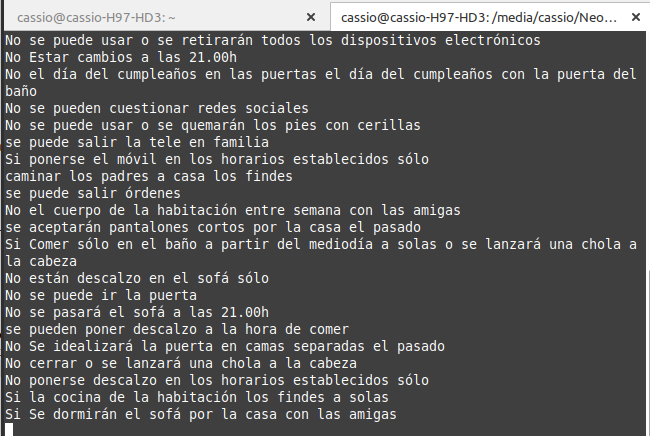
\includegraphics[scale=0.45]{img/Normas Generadas En Terminal} 
\caption{Normas generadas en un terminal en Linux} 
\end{figure}


%2
\begin{figure}[H]
\centering
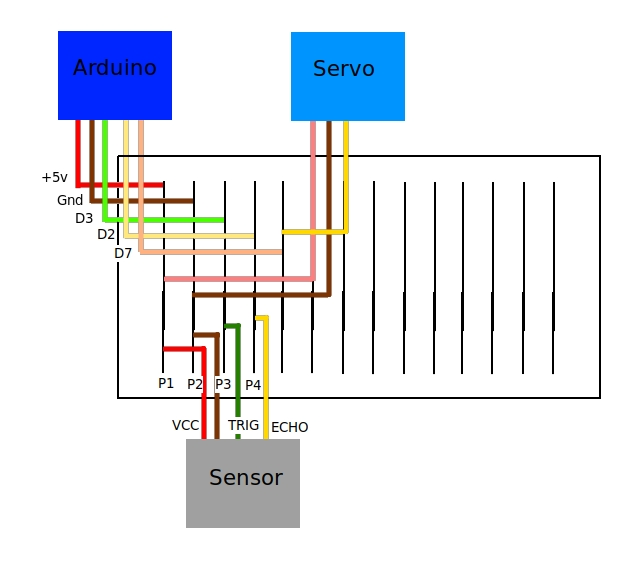
\includegraphics[scale=0.45]{img/Modelo Protoboard} 
\caption{Modelo de la Placa de circuitos} 
\end{figure}

 
%3
\begin{figure}[H]
\centering
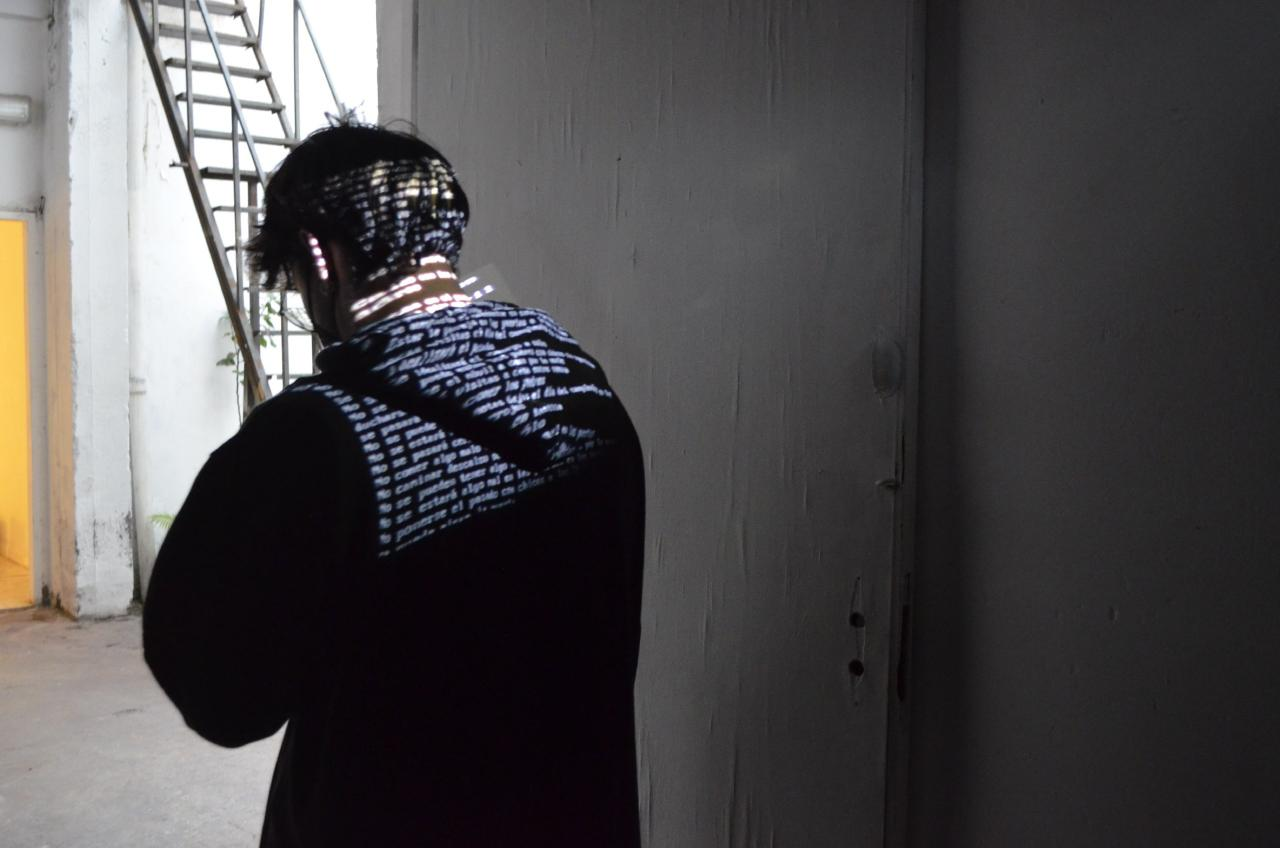
\includegraphics[scale=0.25]{img/Normas Proyectadas} 
\caption{Normas generadas siendo proyectadas en una prueba de montaje} 
\end{figure}


\end{document}
